\documentclass[tikz,border=5pt]{standalone}
\usepackage[UTF8]{ctex}
\usepackage{amsmath,amssymb}
\usetikzlibrary{arrows.meta,calc,angles,quotes,patterns,decorations.pathmorphing}
\definecolor{field}{HTML}{176B9B}
\definecolor{force}{HTML}{B64B32}
\tikzset{>=Latex,line width=.8pt,every node/.style={font=\small},field/.style={color=field},force/.style={color=force},body/.style={draw=black,fill=blue!6},ghost/.style={dashed,gray},labelbox/.style={fill=white,inner sep=1.5pt}}
\begin{document}
\begin{tikzpicture}
% Sphere outline and faint latitude ellipse establish the spatial bowl.
\draw[body](0,0)circle(1.8);
\draw[ghost](0,0)ellipse(1.8 and .45);
\draw[line width=2pt,gray](0,1.8)arc(90:270:1.8);
\foreach\a in{110,135,160,185,210,235,260}
\draw({1.83*cos(\a)},{1.83*sin(\a)})--({2*cos(\a+3)},{2*sin(\a+3)});
\draw[->](-2.2,0)--(3,0)node[right]{$x$};
\draw[->](0,-2.1)--(0,2.3)node[above]{$y$};
\fill(.72,.22)circle(1.6pt)node[above]{$S_0$};
\node[below left]at(0,0){$O$};
\node[left]at(-2.1,.5){镀银面};
\draw[->,field](2.1,.55)--(3.1,.55)node[right]{观察者};
\node at(-.55,-.65){水 $n$};\node at(2.4,-1){空气};
\end{tikzpicture}
\begin{tikzpicture}[xscale=2]
\draw[->](-.2,0)--(2.25,0)node[right]{$x$};
\draw[thick,domain=-1.15:1.15,samples=70]plot({sqrt(4-\x*\x)},\x);
\coordinate(S)at(.86,.16);\coordinate(P)at(1,.187);
\fill(S)circle(.7pt)node[below]{$S_0$};
\fill(P)circle(.7pt)node[above left]{$S_1$};
\foreach\y in{.48,-.35}{
\coordinate(Q)at({sqrt(4-\y*\y)},\y);
\draw[field,->](S)--(Q);
\draw[field,->](Q)--({2.5},{\y+(2.5-sqrt(4-\y*\y))*(\y-.187)/(sqrt(4-\y*\y)-1)});
\draw[ghost](P)--(Q);
}
\draw[force,dashed](0,0)--({sqrt(4-.48*.48)},.48)--(2.5,.618);
\node[force,above]at(1.6,.58){法线 $\beta\simeq y/R$};
\node[below]at(2,-1.3){右顶点 $x=R$};
\node[above]at(.8,1.1){子午截面，一阶近轴光路};
\end{tikzpicture}
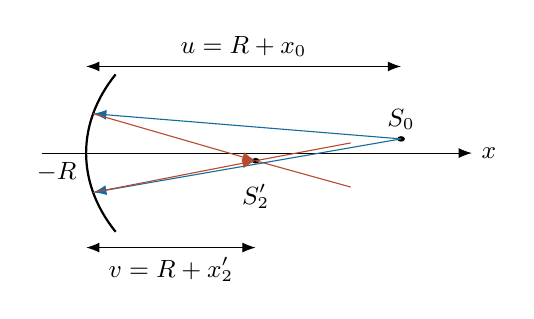
\begin{tikzpicture}[xscale=1.4]
\draw[->](-2.4,0)--(1.5,0)node[right]{$x$};
\draw[thick,domain=-1:1,samples=60]plot({-sqrt(4-\x*\x)},\x);
\coordinate(S)at(.857,.18);\coordinate(I)at(-.462,-.097);
\fill(S)circle(1pt)node[above]{$S_0$};
\fill(I)circle(1pt)node[below=5pt]{$S_2'$};
\foreach\y in{.5,-.5}{
\coordinate(M)at({-sqrt(4-\y*\y)},\y);
\draw[field,->](S)--(M);
\draw[force,->](M)--(I);
\draw[force](I)--({.4},{-.097+(.862)*(-.097-\y)/1.538});
}
\draw[<->](-2,1.1)--(.857,1.1)node[midway,above]{$u=R+x_0$};
\draw[<->](-2,-1.2)--(-.462,-1.2)node[midway,below]{$v=R+x_2'$};
\node[below left]at(-2,0){$-R$};
\end{tikzpicture}
\begin{tikzpicture}[scale=1.5]
\draw[body](0,0)circle(1.8);
\draw[->](-2.1,0)--(2.3,0)node[right]{$x$};
\draw[->](0,-1.8)--(0,2)node[above]{$y$};
\foreach\xx/\yy/\name in {.771/.26/S_0,.9/.303/S_1,-.415/-.14/S_2',-.6/-.202/S_2}{
\fill(\xx,\yy)circle(.7pt);
}
\node at(.42,.85){$S_0$};\draw[gray](.48,.73)--(.771,.26);
\node at(1.12,1.13){$S_1$};\draw[gray](1.07,1.02)--(.9,.303);
\node at(-.23,-.85){$S_2'$};\draw[gray](-.27,-.73)--(-.415,-.14);
\node at(-1,-.6){$S_2$};\draw[gray](-.92,-.5)--(-.6,-.202);
\draw[field,->](.771,.26)--(1.7509997,.42)--(2.25,.4886);
\draw[ghost](.9,.303)--(1.7509997,.42);
\draw[force,->](-.415,-.14)--(1.7549929,-.4)--(2.25,-.4416);
\draw[ghost](-.6,-.202)--(1.7549929,-.4);
\node[below,align=center]at(0,-2.1){示例 $n=4/3$；虚像由出射光线反向延长定位\\轴向按比例，像高为可读性放大};
\end{tikzpicture}
\end{document}
